%**************************************************************
\section{Modular Bayesian Approach}\label{sec:bc_modular_bayes}
%**************************************************************

\lipsum[10]
\begin{figure}[bth]	
	\centering
	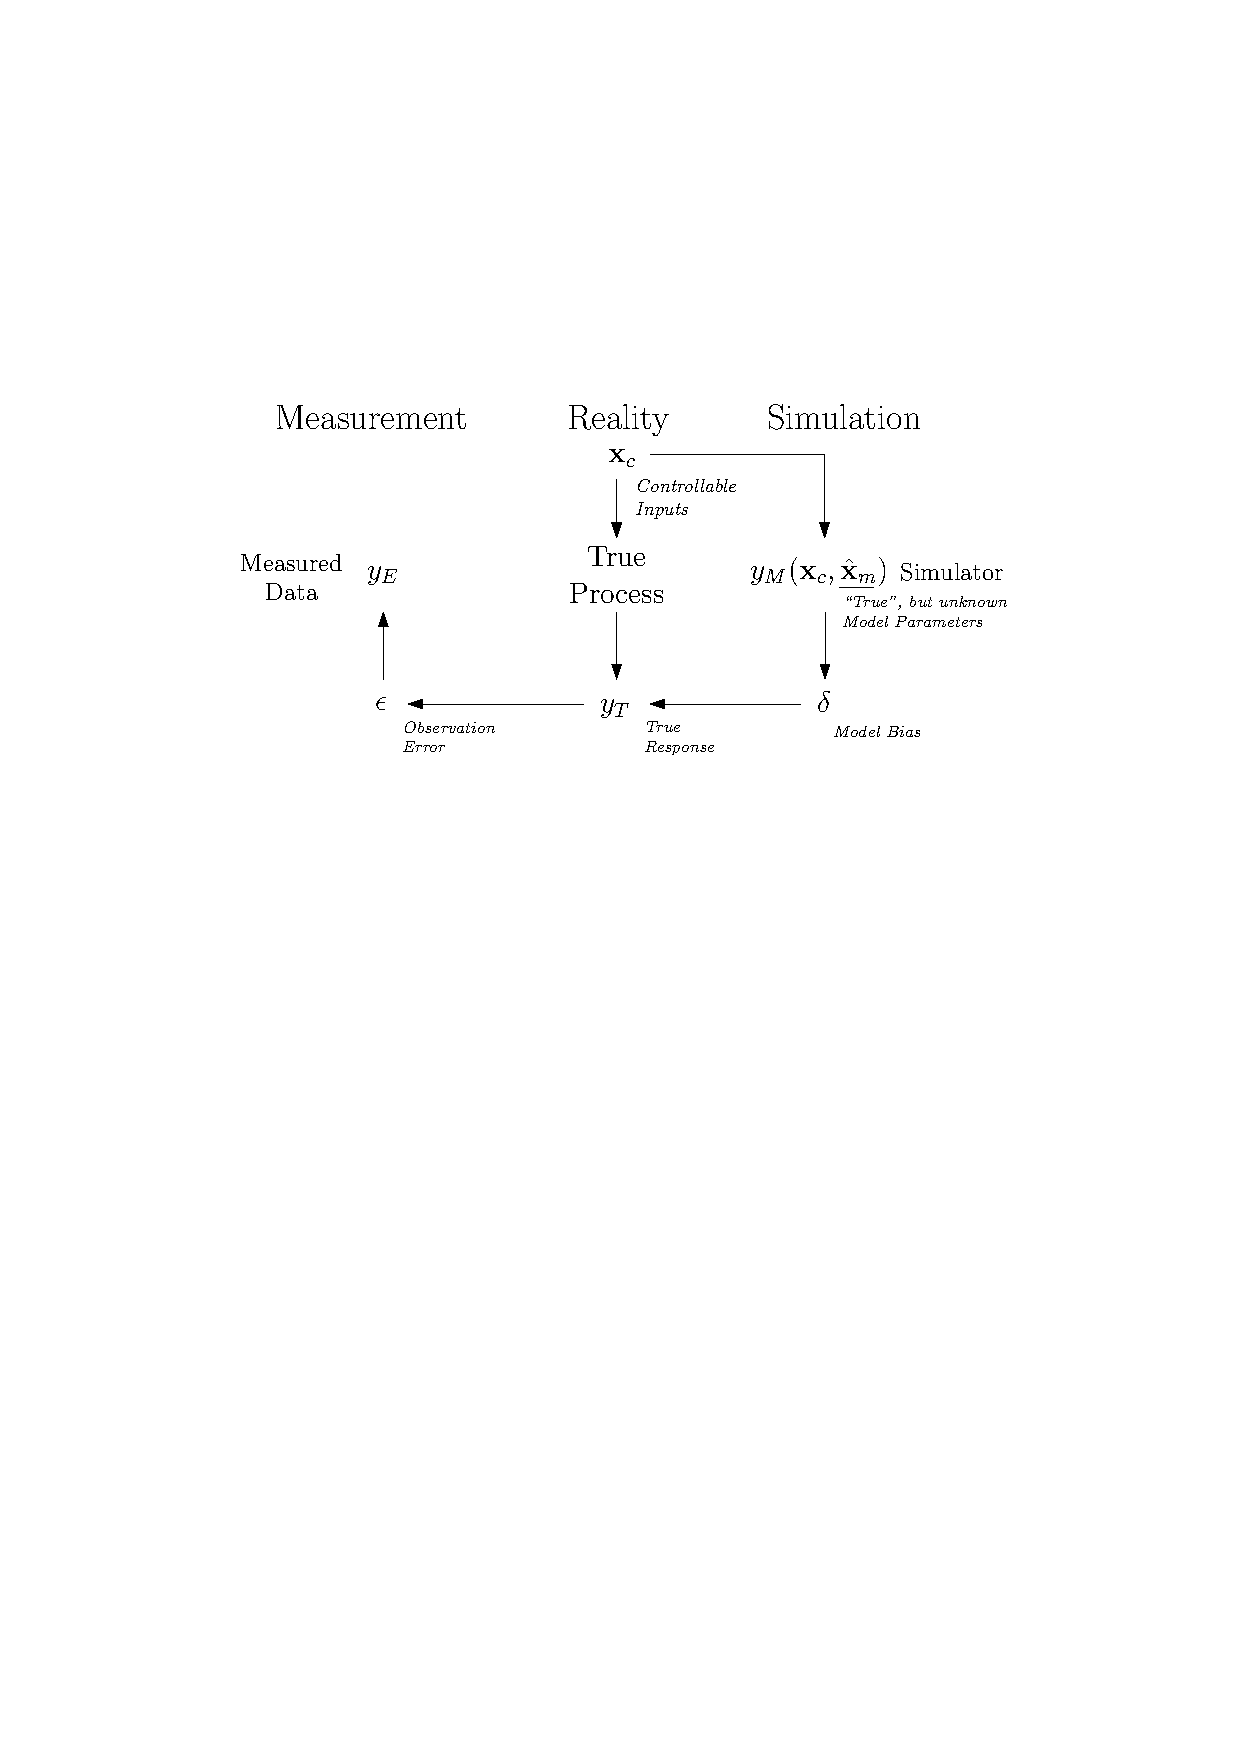
\includegraphics[width=1.0\textwidth]{../figures/chapter5/figures/HMErrorModel}
	\caption[ad]{asd}
	\label{fig:ch5_hm_error_model}
\end{figure}

% Additive formulation
\begin{equation}
    y_E(\bm{x}_c; \lambda) = y_M (\bm{x}_c, \hat{\bm{x}}_m; \lambda) + \delta (\bm{x}_c; \lambda) + \epsilon
\label{eq:bc_additive_formulation}
\end{equation}

% Likelihood
The Bayesian framework begins by constructing a probabilistic model for the data generating process $\mathcal{Y}_E(\bm{x}_c;\lambda)$.
This probabilistic modeling entails casting any uncertain\footnote{here uncertain refers to the state of being imprecise} elements in the equation above as random variable (or in this case, stochastic process). 
\begin{equation}
    \begin{split}
        \mathcal{Y}_M & \equiv \mathcal{Y}_M (\bm{x}_c, \hat{\bm{x}}_m; \lambda) \thicksim  p(y_m | \bm{x}_c, \hat{\bm{x}}_m; \lambda) \\
        (\mathcal{Y}_T - \mathcal{Y}_M) & \equiv \mathcal{D}(\bm{x}_c; \lambda) \thicksim p(\delta | \psi_{\delta}, \bm{x}_c; \lambda) \\
        (\mathcal{Y}_E - \mathcal{Y}_T) & \equiv \mathcal{E}_y(\lambda) \thicksim p(\epsilon_y | \psi_{\epsilon_y}; \lambda) \\
    \end{split}
\label{eq:bc_additive_formulation}
\end{equation}

% Data Generating Process
Under the additive formulation, the data generating process for $\mathcal{Y}_E$ can be obtained by adding all the three terms above.
Assuming those three terms are independent, the \gls[hyper=false]{pdf} of $\mathcal{Y}_E$ is defined as (cite)
\begin{equation}
  p(y_E) = (p(y_m | \bm{x}_c, \hat{\bm{x}}_m; \lambda) * p(\delta | \bm{x}_c; \lambda) * p(\epsilon_y | \lambda))(y_E)
\label{eq:bc_additive_convolution}
\end{equation}
where $*$ is the symbol for convolution operation.

% The Likelihood
The likelihood function is then defined upon 
\begin{equation}
  \mathcal{L}(\hat{\bm{x}}_m, \psi_\delta, \psi_{\epsilon_y}; \mathbf{y}, \mathbf{x}_c, \lambda) \equiv p(y_E = \mathbf{y} | \bm{x}_c = \mathbf{x}_c, \hat{\bm{x}}_m, \psi_\delta, \psi_{\epsilon_y} ; \lambda)
\label{eq:bc_likelihood}
\end{equation}
For conciseness, 
it is always implicitly assumed in the following that a likelihood function is always defined for given data and controllable inputs such that the notation $\mathcal{L}(\hat{\bm{x}}_m, \psi_\delta, \psi_{\epsilon_y}; \lambda)$ is sufficient.

% Full probability model
Following Bayes' theorem, the probability of the model parameters $\bm{x}_m$
\begin{equation}
  p(\bm{x}_m) = \frac{\mathcal{L}(\hat{\bm{x}}_m, \psi_\delta, \psi_{\epsilon_y} ; \lambda) \cdot p(\bm{x}_c) \cdot p(\hat{\bm{x}}_m)\cdot p(\psi_{\epsilon_y}; \lambda) \cdot p(\psi_{\delta})}{\int \mathcal{L}(\hat{\bm{x}}_m, \psi_\delta, \psi_{\epsilon_y}; \lambda) \cdot p(\bm{x}_c) \cdot p(\hat{\bm{x}}_m) p(\psi_{\epsilon_y}) \cdot p(\psi_{\delta}) d\bm{x}_c d\psi_{\epsilon_y} d\psi_\delta}
\label{eq:bc_}
\end{equation}